% Created by tikzDevice version 0.12.3.1 on 2021-06-20 13:38:58
% !TEX encoding = UTF-8 Unicode
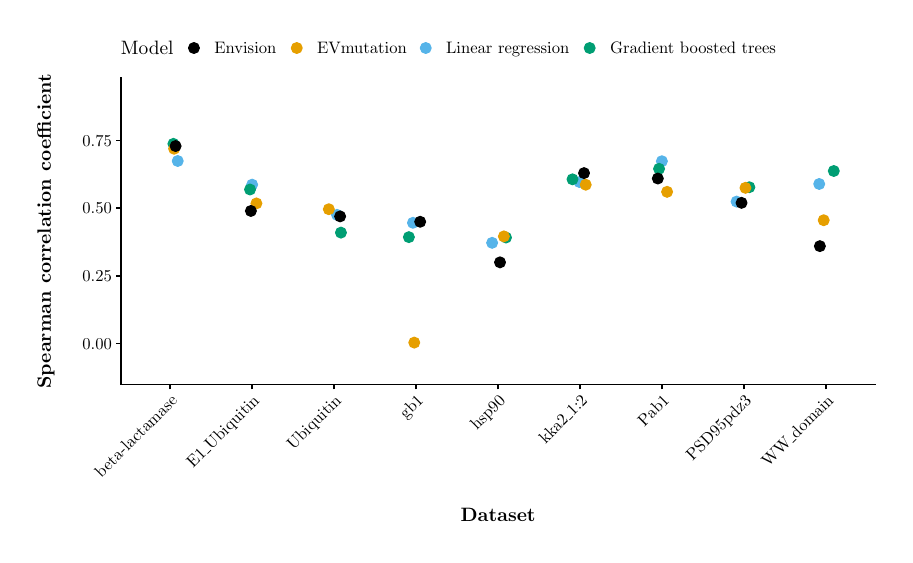
\begin{tikzpicture}[x=1pt,y=1pt]
\definecolor{fillColor}{RGB}{255,255,255}
\path[use as bounding box,fill=fillColor,fill opacity=0.00] (0,0) rectangle (309.84,183.39);
\begin{scope}
\path[clip] ( 33.67, 54.47) rectangle (306.34,165.19);
\definecolor{drawColor}{RGB}{86,180,233}
\definecolor{fillColor}{RGB}{86,180,233}

\path[draw=drawColor,line width= 0.4pt,line join=round,line cap=round,fill=fillColor] ( 54.22,135.21) circle (  1.96);
\definecolor{drawColor}{RGB}{0,158,115}
\definecolor{fillColor}{RGB}{0,158,115}

\path[draw=drawColor,line width= 0.4pt,line join=round,line cap=round,fill=fillColor] ( 52.66,141.41) circle (  1.96);
\definecolor{drawColor}{RGB}{230,159,0}
\definecolor{fillColor}{RGB}{230,159,0}

\path[draw=drawColor,line width= 0.4pt,line join=round,line cap=round,fill=fillColor] ( 52.92,139.63) circle (  1.96);
\definecolor{drawColor}{RGB}{86,180,233}
\definecolor{fillColor}{RGB}{86,180,233}

\path[draw=drawColor,line width= 0.4pt,line join=round,line cap=round,fill=fillColor] ( 81.11,126.66) circle (  1.96);
\definecolor{drawColor}{RGB}{0,158,115}
\definecolor{fillColor}{RGB}{0,158,115}

\path[draw=drawColor,line width= 0.4pt,line join=round,line cap=round,fill=fillColor] ( 80.35,124.91) circle (  1.96);
\definecolor{drawColor}{RGB}{230,159,0}
\definecolor{fillColor}{RGB}{230,159,0}

\path[draw=drawColor,line width= 0.4pt,line join=round,line cap=round,fill=fillColor] ( 82.65,119.88) circle (  1.96);
\definecolor{drawColor}{RGB}{86,180,233}
\definecolor{fillColor}{RGB}{86,180,233}

\path[draw=drawColor,line width= 0.4pt,line join=round,line cap=round,fill=fillColor] (111.78,115.75) circle (  1.96);
\definecolor{drawColor}{RGB}{0,158,115}
\definecolor{fillColor}{RGB}{0,158,115}

\path[draw=drawColor,line width= 0.4pt,line join=round,line cap=round,fill=fillColor] (113.20,109.33) circle (  1.96);
\definecolor{drawColor}{RGB}{230,159,0}
\definecolor{fillColor}{RGB}{230,159,0}

\path[draw=drawColor,line width= 0.4pt,line join=round,line cap=round,fill=fillColor] (108.82,117.79) circle (  1.96);
\definecolor{drawColor}{RGB}{86,180,233}
\definecolor{fillColor}{RGB}{86,180,233}

\path[draw=drawColor,line width= 0.4pt,line join=round,line cap=round,fill=fillColor] (139.22,112.88) circle (  1.96);
\definecolor{drawColor}{RGB}{0,158,115}
\definecolor{fillColor}{RGB}{0,158,115}

\path[draw=drawColor,line width= 0.4pt,line join=round,line cap=round,fill=fillColor] (137.75,107.70) circle (  1.96);
\definecolor{drawColor}{RGB}{230,159,0}
\definecolor{fillColor}{RGB}{230,159,0}

\path[draw=drawColor,line width= 0.4pt,line join=round,line cap=round,fill=fillColor] (139.69, 69.59) circle (  1.96);
\definecolor{drawColor}{RGB}{86,180,233}
\definecolor{fillColor}{RGB}{86,180,233}

\path[draw=drawColor,line width= 0.4pt,line join=round,line cap=round,fill=fillColor] (167.83,105.64) circle (  1.96);
\definecolor{drawColor}{RGB}{0,158,115}
\definecolor{fillColor}{RGB}{0,158,115}

\path[draw=drawColor,line width= 0.4pt,line join=round,line cap=round,fill=fillColor] (172.84,107.55) circle (  1.96);
\definecolor{drawColor}{RGB}{230,159,0}
\definecolor{fillColor}{RGB}{230,159,0}

\path[draw=drawColor,line width= 0.4pt,line join=round,line cap=round,fill=fillColor] (172.08,107.97) circle (  1.96);
\definecolor{drawColor}{RGB}{86,180,233}
\definecolor{fillColor}{RGB}{86,180,233}

\path[draw=drawColor,line width= 0.4pt,line join=round,line cap=round,fill=fillColor] (199.41,127.60) circle (  1.96);
\definecolor{drawColor}{RGB}{0,158,115}
\definecolor{fillColor}{RGB}{0,158,115}

\path[draw=drawColor,line width= 0.4pt,line join=round,line cap=round,fill=fillColor] (196.87,128.59) circle (  1.96);
\definecolor{drawColor}{RGB}{230,159,0}
\definecolor{fillColor}{RGB}{230,159,0}

\path[draw=drawColor,line width= 0.4pt,line join=round,line cap=round,fill=fillColor] (201.65,126.64) circle (  1.96);
\definecolor{drawColor}{RGB}{86,180,233}
\definecolor{fillColor}{RGB}{86,180,233}

\path[draw=drawColor,line width= 0.4pt,line join=round,line cap=round,fill=fillColor] (229.17,135.13) circle (  1.96);
\definecolor{drawColor}{RGB}{0,158,115}
\definecolor{fillColor}{RGB}{0,158,115}

\path[draw=drawColor,line width= 0.4pt,line join=round,line cap=round,fill=fillColor] (228.15,132.39) circle (  1.96);
\definecolor{drawColor}{RGB}{230,159,0}
\definecolor{fillColor}{RGB}{230,159,0}

\path[draw=drawColor,line width= 0.4pt,line join=round,line cap=round,fill=fillColor] (231.05,124.07) circle (  1.96);
\definecolor{drawColor}{RGB}{86,180,233}
\definecolor{fillColor}{RGB}{86,180,233}

\path[draw=drawColor,line width= 0.4pt,line join=round,line cap=round,fill=fillColor] (256.16,120.54) circle (  1.96);
\definecolor{drawColor}{RGB}{0,158,115}
\definecolor{fillColor}{RGB}{0,158,115}

\path[draw=drawColor,line width= 0.4pt,line join=round,line cap=round,fill=fillColor] (260.78,125.74) circle (  1.96);
\definecolor{drawColor}{RGB}{230,159,0}
\definecolor{fillColor}{RGB}{230,159,0}

\path[draw=drawColor,line width= 0.4pt,line join=round,line cap=round,fill=fillColor] (259.36,125.51) circle (  1.96);
\definecolor{drawColor}{RGB}{86,180,233}
\definecolor{fillColor}{RGB}{86,180,233}

\path[draw=drawColor,line width= 0.4pt,line join=round,line cap=round,fill=fillColor] (286.02,126.91) circle (  1.96);
\definecolor{drawColor}{RGB}{0,158,115}
\definecolor{fillColor}{RGB}{0,158,115}

\path[draw=drawColor,line width= 0.4pt,line join=round,line cap=round,fill=fillColor] (291.29,131.60) circle (  1.96);
\definecolor{drawColor}{RGB}{230,159,0}
\definecolor{fillColor}{RGB}{230,159,0}

\path[draw=drawColor,line width= 0.4pt,line join=round,line cap=round,fill=fillColor] (287.64,113.81) circle (  1.96);
\definecolor{drawColor}{RGB}{0,0,0}
\definecolor{fillColor}{RGB}{0,0,0}

\path[draw=drawColor,line width= 0.4pt,line join=round,line cap=round,fill=fillColor] ( 53.45,140.61) circle (  1.96);

\path[draw=drawColor,line width= 0.4pt,line join=round,line cap=round,fill=fillColor] (227.70,128.88) circle (  1.96);

\path[draw=drawColor,line width= 0.4pt,line join=round,line cap=round,fill=fillColor] ( 80.66,117.16) circle (  1.96);

\path[draw=drawColor,line width= 0.4pt,line join=round,line cap=round,fill=fillColor] (201.04,130.84) circle (  1.96);

\path[draw=drawColor,line width= 0.4pt,line join=round,line cap=round,fill=fillColor] (257.96,120.09) circle (  1.96);

\path[draw=drawColor,line width= 0.4pt,line join=round,line cap=round,fill=fillColor] (286.26,104.45) circle (  1.96);

\path[draw=drawColor,line width= 0.4pt,line join=round,line cap=round,fill=fillColor] (112.90,115.20) circle (  1.96);

\path[draw=drawColor,line width= 0.4pt,line join=round,line cap=round,fill=fillColor] (141.83,113.25) circle (  1.96);

\path[draw=drawColor,line width= 0.4pt,line join=round,line cap=round,fill=fillColor] (170.68, 98.59) circle (  1.96);
\end{scope}
\begin{scope}
\path[clip] (  0.00,  0.00) rectangle (309.84,183.39);
\definecolor{drawColor}{RGB}{0,0,0}

\path[draw=drawColor,line width= 0.6pt,line join=round,line cap=rect] ( 33.67, 54.47) --
	( 33.67,165.19);
\end{scope}
\begin{scope}
\path[clip] (  0.00,  0.00) rectangle (309.84,183.39);
\definecolor{drawColor}{RGB}{0,0,0}

\node[text=drawColor,anchor=base east,inner sep=0pt, outer sep=0pt, scale=  0.60] at ( 30.42, 67.21) {0.00};

\node[text=drawColor,anchor=base east,inner sep=0pt, outer sep=0pt, scale=  0.60] at ( 30.42, 91.64) {0.25};

\node[text=drawColor,anchor=base east,inner sep=0pt, outer sep=0pt, scale=  0.60] at ( 30.42,116.07) {0.50};

\node[text=drawColor,anchor=base east,inner sep=0pt, outer sep=0pt, scale=  0.60] at ( 30.42,140.50) {0.75};
\end{scope}
\begin{scope}
\path[clip] (  0.00,  0.00) rectangle (309.84,183.39);
\definecolor{drawColor}{RGB}{0,0,0}

\path[draw=drawColor,line width= 0.6pt,line join=round] ( 31.92, 69.28) --
	( 33.67, 69.28);

\path[draw=drawColor,line width= 0.6pt,line join=round] ( 31.92, 93.71) --
	( 33.67, 93.71);

\path[draw=drawColor,line width= 0.6pt,line join=round] ( 31.92,118.14) --
	( 33.67,118.14);

\path[draw=drawColor,line width= 0.6pt,line join=round] ( 31.92,142.57) --
	( 33.67,142.57);
\end{scope}
\begin{scope}
\path[clip] (  0.00,  0.00) rectangle (309.84,183.39);
\definecolor{drawColor}{RGB}{0,0,0}

\path[draw=drawColor,line width= 0.6pt,line join=round,line cap=rect] ( 33.67, 54.47) --
	(306.34, 54.47);
\end{scope}
\begin{scope}
\path[clip] (  0.00,  0.00) rectangle (309.84,183.39);
\definecolor{drawColor}{RGB}{0,0,0}

\path[draw=drawColor,line width= 0.6pt,line join=round] ( 51.45, 52.72) --
	( 51.45, 54.47);

\path[draw=drawColor,line width= 0.6pt,line join=round] ( 81.09, 52.72) --
	( 81.09, 54.47);

\path[draw=drawColor,line width= 0.6pt,line join=round] (110.73, 52.72) --
	(110.73, 54.47);

\path[draw=drawColor,line width= 0.6pt,line join=round] (140.37, 52.72) --
	(140.37, 54.47);

\path[draw=drawColor,line width= 0.6pt,line join=round] (170.00, 52.72) --
	(170.00, 54.47);

\path[draw=drawColor,line width= 0.6pt,line join=round] (199.64, 52.72) --
	(199.64, 54.47);

\path[draw=drawColor,line width= 0.6pt,line join=round] (229.28, 52.72) --
	(229.28, 54.47);

\path[draw=drawColor,line width= 0.6pt,line join=round] (258.92, 52.72) --
	(258.92, 54.47);

\path[draw=drawColor,line width= 0.6pt,line join=round] (288.55, 52.72) --
	(288.55, 54.47);
\end{scope}
\begin{scope}
\path[clip] (  0.00,  0.00) rectangle (309.84,183.39);
\definecolor{drawColor}{RGB}{0,0,0}

\node[text=drawColor,rotate= 45.00,anchor=base east,inner sep=0pt, outer sep=0pt, scale=  0.60] at ( 54.38, 48.30) {beta-lactamase};

\node[text=drawColor,rotate= 45.00,anchor=base east,inner sep=0pt, outer sep=0pt, scale=  0.60] at ( 84.01, 48.30) {E1\_Ubiquitin};

\node[text=drawColor,rotate= 45.00,anchor=base east,inner sep=0pt, outer sep=0pt, scale=  0.60] at (113.65, 48.30) {Ubiquitin};

\node[text=drawColor,rotate= 45.00,anchor=base east,inner sep=0pt, outer sep=0pt, scale=  0.60] at (143.29, 48.30) {gb1};

\node[text=drawColor,rotate= 45.00,anchor=base east,inner sep=0pt, outer sep=0pt, scale=  0.60] at (172.93, 48.30) {hsp90};

\node[text=drawColor,rotate= 45.00,anchor=base east,inner sep=0pt, outer sep=0pt, scale=  0.60] at (202.56, 48.30) {kka2\_1:2};

\node[text=drawColor,rotate= 45.00,anchor=base east,inner sep=0pt, outer sep=0pt, scale=  0.60] at (232.20, 48.30) {Pab1};

\node[text=drawColor,rotate= 45.00,anchor=base east,inner sep=0pt, outer sep=0pt, scale=  0.60] at (261.84, 48.30) {PSD95pdz3};

\node[text=drawColor,rotate= 45.00,anchor=base east,inner sep=0pt, outer sep=0pt, scale=  0.60] at (291.48, 48.30) {WW\_domain};
\end{scope}
\begin{scope}
\path[clip] (  0.00,  0.00) rectangle (309.84,183.39);
\definecolor{drawColor}{RGB}{0,0,0}

\node[text=drawColor,anchor=base,inner sep=0pt, outer sep=0pt, scale=  0.70] at (170.00,  4.86) {\bfseries Dataset};
\end{scope}
\begin{scope}
\path[clip] (  0.00,  0.00) rectangle (309.84,183.39);
\definecolor{drawColor}{RGB}{0,0,0}

\node[text=drawColor,rotate= 90.00,anchor=base,inner sep=0pt, outer sep=0pt, scale=  0.70] at (  8.39,109.83) {\bfseries Spearman correlation coefficient};
\end{scope}
\begin{scope}
\path[clip] (  0.00,  0.00) rectangle (309.84,183.39);
\definecolor{drawColor}{RGB}{0,0,0}

\node[text=drawColor,anchor=base west,inner sep=0pt, outer sep=0pt, scale=  0.70] at ( 33.67,173.63) {Model};
\end{scope}
\begin{scope}
\path[clip] (  0.00,  0.00) rectangle (309.84,183.39);
\definecolor{drawColor}{RGB}{0,0,0}
\definecolor{fillColor}{RGB}{0,0,0}

\path[draw=drawColor,line width= 0.4pt,line join=round,line cap=round,fill=fillColor] ( 60.08,176.04) circle (  1.96);
\end{scope}
\begin{scope}
\path[clip] (  0.00,  0.00) rectangle (309.84,183.39);
\definecolor{drawColor}{RGB}{230,159,0}
\definecolor{fillColor}{RGB}{230,159,0}

\path[draw=drawColor,line width= 0.4pt,line join=round,line cap=round,fill=fillColor] ( 97.23,176.04) circle (  1.96);
\end{scope}
\begin{scope}
\path[clip] (  0.00,  0.00) rectangle (309.84,183.39);
\definecolor{drawColor}{RGB}{86,180,233}
\definecolor{fillColor}{RGB}{86,180,233}

\path[draw=drawColor,line width= 0.4pt,line join=round,line cap=round,fill=fillColor] (143.84,176.04) circle (  1.96);
\end{scope}
\begin{scope}
\path[clip] (  0.00,  0.00) rectangle (309.84,183.39);
\definecolor{drawColor}{RGB}{0,158,115}
\definecolor{fillColor}{RGB}{0,158,115}

\path[draw=drawColor,line width= 0.4pt,line join=round,line cap=round,fill=fillColor] (203.08,176.04) circle (  1.96);
\end{scope}
\begin{scope}
\path[clip] (  0.00,  0.00) rectangle (309.84,183.39);
\definecolor{drawColor}{RGB}{0,0,0}

\node[text=drawColor,anchor=base west,inner sep=0pt, outer sep=0pt, scale=  0.60] at ( 67.43,173.97) {Envision};
\end{scope}
\begin{scope}
\path[clip] (  0.00,  0.00) rectangle (309.84,183.39);
\definecolor{drawColor}{RGB}{0,0,0}

\node[text=drawColor,anchor=base west,inner sep=0pt, outer sep=0pt, scale=  0.60] at (104.58,173.97) {EVmutation};
\end{scope}
\begin{scope}
\path[clip] (  0.00,  0.00) rectangle (309.84,183.39);
\definecolor{drawColor}{RGB}{0,0,0}

\node[text=drawColor,anchor=base west,inner sep=0pt, outer sep=0pt, scale=  0.60] at (151.19,173.97) {Linear regression};
\end{scope}
\begin{scope}
\path[clip] (  0.00,  0.00) rectangle (309.84,183.39);
\definecolor{drawColor}{RGB}{0,0,0}

\node[text=drawColor,anchor=base west,inner sep=0pt, outer sep=0pt, scale=  0.60] at (210.43,173.97) {Gradient boosted trees};
\end{scope}
\end{tikzpicture}
